\documentclass[a4paper,12pt]{article}
\usepackage[margin=0.7in]{geometry}
\usepackage[latin1]{inputenc}
\usepackage[english]{babel}
\usepackage{amsmath}
\usepackage{cases}
\usepackage[makeroom]{cancel}
\usepackage{amsmath,tabu}
\usepackage[fleqn]{mathtools}
\usepackage[fleqn]{amsmath}
\usepackage{bm}
\usepackage{tikz}
\usepackage{enumitem}
\usepackage{wrapfig}
\usepackage{graphicx}
\usepackage{siunitx}
\usepackage{microtype}
\usepackage{array,tabularx}
\usepackage{float}
\usepackage{booktabs}
\usepackage{import}
\usepackage{cases}
\usepackage{graphicx,subfigure}
\usepackage{myUnitOfMeasure}
%\usepackage{myThermodynamics}
\usepackage{myMath}
\usepackage{mathtools}
\usepackage{gensymb}
\usepackage{xcolor}

\title{PROJECT 3: Design of a Pressure Vessel}
\author{Rossi Andrea 883580}
\date{}


\DeclarePairedDelimiter\abs{\lvert}{\rvert}%

\newcommand{\Fy}[1]{\text{F}_{y_{#1}}}

\newcommand{\diameter}{\oslash}

\newcommand{\todo}{\colorbox{cyan!60}{TODO}}

\renewcommand{\thesubsection}{\thesection.\arabic{subsection}}

\begin{document}
%\tableofcontents
\maketitle

\section{Fatigue Design of a Pressure Vessel}

\subsection{Introduction to the problem}


The report consists in the design of a \emph{pressure vessel having a cylindrical shell and hemispheric ends} through the comparison between:
\begin{itemize}
\item the static assessment, computed by using the Mariotte's formulation;
\item the analytical calculation of the fatigue life, adopting Mariotte's formulation;
\item a simulation with finite element.
\end{itemize} 

The simulation is performed with the support of the software Abaqus.

\begin{figure}[H]
\centering
\includegraphics[width=0.6\textwidth]{img/slides/Basic_vessel.png}
\caption{Pressure Vessel example.}
\label{fig:Vessel_example}
\end{figure}

A pressure vessel is a container designed to hold gases or liquids at a pressure substantially different from the ambient pressure.
The pressure differential is dangerous, and fatal accidents have occurred in the history of pressure vessel development and operation. Consequently, pressure vessel design, manufacture, and operation are regulated by engineering authorities.

In our case study, the vessel is filled up with a pressurize gas and it has the following characteristics:
\begin{itemize}
\item Ultimate tensile strength,UTS, equal to 1000 MPa;
\item Yielding stress, YS, equal to 900 MPa;
\item Internal pressure,Pw , equal to 200 bar.
\end{itemize}

And its dimensions are:
\begin{itemize}
\item Outer shell diameter, D , equal to 230 mm;
\item Shell thickness, t, equal to 5.8 mm;
\item Half the length of the cylindrical shell, L, equal to 250 mm.
\end{itemize}

\begin{figure}[H]
\centering
\includegraphics[width=0.7\textwidth]{img/slides/rappre.png}
\caption{Pressure Vesssel schematization.}
\label{fig:Vessel_scheme}
\end{figure}



\subsection{Static Assessment}

In order to perform the static assessment of the vessel in the cylindrical shell, far from the borders, we decided to use the Mariotte's solution for small thickness cylinder.

Then, for our calculation we have used as pressure two times the nominal one, so that we are taking the safety factor directly on the input instead of on the output as usually.
So, the following stresses are present:

 \begin{equation}
\sigma_{axial} = \dfrac{P_w \, d_{\text{internal}}}{ 4 \, t} = \round{376.5517} \MPa
\label{sigma_axial}
\end{equation}

\begin{equation}
\sigma_{circumferenzial} = \dfrac{P_w \, d_{\text{internal}}}{ 2 \, t} = \round{753.1034} \MPa
\label{sigma_circ}
\end{equation}
 \begin{equation}
\sigma_{radial} = -P_w = \round{-40} \MPa
\label{sigma_rad}
\end{equation}

After the computation of the stresses, we have moved our attention on the calculation of the Guest-Tresca's stress in order to apply the correspondent criterion. The $\sigma_{GT}$ results:

\begin{equation}
\sigma_{guest-tresca} = |\sigma_{max}-\sigma_{min}| = \round{793.1034} \MPa
\label{guest_tres_static}
\end{equation}

Finally, we have evaluated the safety factor of the static assessment. We have to remember that to have a safe component, the $\eta$ should be simply greater than 1 since we have taken already a safety factor of 2 applying the pressure.  

\begin{equation}
\eta = \dfrac{ YS }{ \sigma_{guest-tresca} } = \round{1.1348}
\label{safety_static}
\end{equation}
In conclusion, as it is visible form equation \ref{safety_static}, the component is able to pass the static assessment.

\subsection{Fatigue assessment - Analytical}

In order to perform the analytical fatigue assessment of the vessel in the cylindrical shell, far from the borders, we decided to use the Mariotte's solution for small thickness cylinder.
But despite from the static assessment, here we have consider a value of pressure  which is fifty percent more than the nominal pressure. 

The pressure on the inner shell surface is pulsing, as it is shown in the following figure \ref{fig:pres-var}:

\begin{figure}[H]
\centering
\includegraphics[width=0.5\textwidth]{img/slides/pres_variation.png}
\caption{Pressure variation inside the Vessel.}
\label{fig:pres-var}
\end{figure}

The standard requirements states that the component must have a minimum life span of 12000 cycles.

The component must resist to radial, axial and hoop stresses, so it is in a multi-axial load condition. In this case the proper approach to use is the Sines criterion. 

Since we have to deal with multi-axial fatigue loads, the stress components have to be split into two components, one mean and one alternated. The criterion that we have chosen states that:
\begin{equation}
\sigma_{AR} = \dfrac{\sigma^\star}{1-\dfrac{\text{I}_m}{\text{UTS}}} < \dfrac{\sigma'_e}{\eta}
\end{equation}
\begin{conditions}
\sigma^\star & Sines equivalent stress;\\[0.5em]
\text{I}_m & first stress invariant;\\[0.5em]
\text{UTS} & ultimate tensile strength;\\[0.5em]
\sigma'_e & endurance limit of the mechanical component;\\[0.5em]
\eta & safety factor.\\[0.5em]
\end{conditions}
We can express the previous quantities as function of material and geometrical properties and mean and alternated stresses. In fact,
the Sines equivalent stress only considers the alternated component of the stresses and is equal to:
\begin{equation}
\sigma^\star = \sqrt{\text{S}_{x_a}^2 + \text{S}_{y_a}^2 + \text{S}_{z_a}^2
- \text{S}_{x_a} \, \text{S}_{y_a} - \text{S}_{x_a} \, \text{S}_{z_a} - \text{S}_{y_a} \, \text{S}_{z_a}
+ 3\, \tau_{xy_a}^2 + 3\, \tau_{xz_a}^2 + 3\, \tau_{yz_a}^2 }
\end{equation}
The first invariant stress instead is only taking into account the mean stress and it is defined as the sum of the principal mean stresses.
\begin{equation}
\text{I}_m = \text{S}_{x_m} + \text{S}_{y_m} + \text{S}_{z_m}
\label{eq:first_invariant}
\end{equation}
The endurance limit instead depends mainly on the material resistance but it can be reduces a lot when the component is really different from the standard specimen in term of dimensions ($\text{m}_d$), surface finishing ($\text{m}_s$) and presence of notch ($\text{k}_f$):
\begin{equation}
\sigma'_e = \dfrac{\sigma_e \, \text{m}_s \, \text{m}_d}{\text{k}_f}
\end{equation}
Where:
\begin{itemize}
\item $\sigma_e = 0.4\, \text{UTS}$ in axial alternated fatigue;
\item the dimensional effect $\text{m}_d$ is set to 1 because the stress state is constant through the thickness and therefore there is no stress gradient;
\item the surface effect $\text{m}_s$ is equal to 0.7, as a typical value;
\item the fatigue notch factor $\text{K}_f$ equals to 1 because there is no notch.
\end{itemize}

As hypothesis it states that all the stress components have to be synchronous and with the same phase.
All the stresses have the same frequency, but the radial one is always of compression, so it is pulsating and negative.

So, we have to perform a simple modification to the Sines criterion (in order to be able to take into account the 180 degree phase difference) by calculating the equivalent stress as states in the following equation:
\begin{equation}
\sigma^\star = \sqrt{\text{S}_{a_a}^2 + \text{S}_{t_a}^2 + \text{S}_{t_a}^2
- \text{S}_{a_a} \, \text{S}_{t_a} 
+ \text{S}_{t_a} \, \text{S}_{r_a} 
+ \text{S}_{a_a} \, \text{S}_{r_a}}
\label{eq:sigma_star}
\end{equation}
Moreover as it appears in equation \ref{eq:sigma_star}, we have neglected the tangential stresses because in the Mariotte's formulation the results are directly the principal stresses.
Now, we have to compute mean and alternated stresses calculation. Since the loads are pulsating the absolute value of two components is the same. The results are reported in table \ref{table:fatigue_principal_stresses}.


\begin{table}[H]
\centering
\caption{Fatigue principal stresses}
\label{table:fatigue_principal_stresses}
\begin{tabular}{@{}lcc@{}}
\toprule
                & Mean                                  & Alternated                            \\ \midrule
Axial           & $\round{1.412068965517241e+02} \MPa $ & $\round{1.412068965517241e+02} \MPa $ \\
Circumferential & $\round{2.824137931034483e+02} \MPa $ & $\round{2.824137931034483e+02} \MPa $ \\
Radial          & $\round{-15} \MPa $                   & $\round{15} \MPa $                    \\ \bottomrule
\end{tabular}
\end{table}

After this, we can calculate the Sines equivalent stress with equation \ref{eq:sigma_star} and the first invariant with equation \ref{eq:first_invariant}:
\begin{equation}
\sigma^\star = \sqrt{\text{S}_{a_a}^2 + \text{S}_{t_a}^2 + \text{S}_{t_a}^2
- \text{S}_{a_a} \, \text{S}_{t_a} 
+ \text{S}_{t_a} \, \text{S}_{r_a} 
+ \text{S}_{a_a} \, \text{S}_{r_a}}
= \round{257.6771} \MPa
\label{eq:sigma_star_value}
\end{equation}
\begin{equation}
\text{I}_m = \text{S}_{r_m} + \text{S}_{t_m} + \text{S}_{a_m}
= \round{408.6207} \MPa
\label{eq:first_invariant_value}
\end{equation}

To enter in the Wohler diagram for getting the number of cycles equivalent to a certain stress, we have to find an equivalent fully reversed stress to our multi-axial configuration. This is the key point of the Sines criterion, which provide us a simple formula to apply this conversion:
\begin{equation}
\sigma_{AR} = \dfrac{\sigma^\star}{1-\dfrac{\text{I}_m}{\text{UTS}}}
= \round{435.7222} \MPa
\label{eq:sigma_AR}
\end{equation}


 
 After the computation of the equivalent fully reversed stress, $\sigma_{AR}$ , we are able to find the maximum number of cycles at which the vessel fails and , also, to verify if this value is higher than the minimum request of the standard, $\text{N}=12000 $ cycles.
For doing those tasks, we have entered into the Wohler curve with the value of $\sigma_{AR}$, which is reported in the equation \ref{eq:sigma_AR}. 

The Wohler curve, as shown in the figure \ref{fig:wohler_base}, represents the relationship between the stress amplitude and the number of cycles to failure, in particular it is a straight line in the finite-life region. For having a simplified curve representation, we plot the curve in a log-log plane, as it is shown in figure \ref{fig:wohler_base}.

\begin{figure}[H]
\centering
\includegraphics[width=0.6\textwidth]{img/slides/wohler.png}
\caption{Wohler curve.}
\label{fig:wohler_base}
\end{figure}

In our analysis, we have used the following curve, in which are already reported the values of the points, that are going to be used for our calculation:

\begin{figure}[H]
\centering
\includegraphics[width=0.6\textwidth]{img/slides/proje_whol.png}
\caption{Wohler curve for our case study.}
\label{fig:wohler_precise}
\end{figure}

In fact, the S-N Wohler curve has as function the following equation:
\begin{equation}
\sigma = {\text{A}}{\text{N}^B}
\label{eq:equa-woh}
\end{equation}
%
And it is drawn based on the two points, which are represented in the figure \ref{fig:wohler_precise}.
In order to the plot the curve, we have to find the parameters present in the equation \ref{eq:equa-woh}, simply considering that point 1 and point 2 belong to the curve; so, we obtain the following system:

\begin{align}
\begin{cases}{}
\text{S}_1 = \log A + B\, \log \text{N}_1 \\[0.5em]
\text{S}_2 = \log A + B\, \log \text{N}_2 
\end{cases}
\end{align}

and we obtain that:

\begin{equation}
\text{B}=\dfrac{\log{\dfrac{\text{S}_2}{\text{S}_1}}}{\log{\dfrac{\text{N}_2}{\text{N}_1}}}= \round{-0.137088021125527}
\end{equation}

\begin{equation}
\text{A} = \dfrac{\text{S}_1}{\text{N}_1^B}= \round{2.320099298772334e+03} \MPa
\end{equation}
Now that we know the parameters of the curve, we are able to find the number of cycle for the component.
In general, we have to remember that also for the number of cycles there is a safety coefficient, since the "safe-life" approach in evaluating a limit number of cycles. This coefficient is commonly considered acceptable when is grater than 4 or 6.\\
In our case study, we do not have to consider this coefficient, since we are already working with a pressure which is higher than the service one (in fact, the pressure value is fifty percent grater than the nominal value).
So, the only thing which we have to care about is if the number of cycles evaluated is greater or equal to the target one.\\
The analytical number found is reported in the following equation:

\begin{equation}
\text{N}_f= \round{1.986247944207594e+05} = \round[round-precision=0]{1.986247944207594e+05 - 0.5}
\end{equation}

As it is clearly visible the value found is more or less fifteen times grater than the target.


\subsection{Numerical Analysis}


In order to perform the numerical analysis on the pressure vessel, we have created a model into the simulation software Abaqus.\\ Our attention has been focused on the best way to describe a pressure vessel; on this way, we have decided (taking into account the dimensions given into the drawings and the geometry of the vessel) to use an axis-symmetric model and to evaluate the stresses only into a tiny slice of our vessel, in order to reduce the computational cost. \\For doing this, we have focused our attention to the real vessel: being it symmetrical in the Y direction, it would be meaningless to perform the whole analysis for the pressure vessel instead of a simulation on one half of the geometry.\\ Here below is reported a sketched, which represent our modelization:

\begin{figure}[H]
\centering
\includegraphics[width=0.5\textwidth]{img/schem.png}
\caption{Abaqus model.}
\end{figure}


At this point we have set the load and the boundary conditions. The pressure has been set constant along the geometry and 1.5 times the real pressure inside the vessel, in order to have, before the simulation, a sort of safety factor inside the model itself. Then, as buondary condition we have place a constraint for the symmetry in the Y direction.\\ Right below is reported the load and constrained model: 
\begin{figure}[H]
\centering
\includegraphics[width=0.5\textwidth]{img/conload.png}
\caption{Constrained and Loaded model.}
\end{figure}

Moreover, the geometry of the component can be approximated with an hollow cylinder with thin walls; so, we have decided to use solid finite elements instead of shell ones, in order to avoid errors and/or over-estimation of the values in correspondence of the interfaces and changes of geometry. \\
According to the standards, we have imposed at least a minimum number of finite elements into the thickness, for being able to investigate in the correct way the behaviour of the stresses along the internal and external surfaces.\\
Another important point along the development of the model has been played by the choice of the type of the Finite Elements. Actually, being the model axis-symmetric, also the elements must be right that: for this reason, we have used the antisymmetric quadratic elements with 8 nodes each.\\


After running the simulation, we have compared the results of the analysis between the inner and outer wall of the vessel, in order to assess which of the two is the most stressed section.
To do this we calculated the safety coefficient and we looked at the lowest point, as reported in the following diagrams:

\begin{figure}[H]
\centering     %%% not \center
\caption{Safety Coefficient for the Inner and Outer wall of the vessel.}
\subfigure[Inner Safety Coefficient]{\label{fig:a}\includegraphics[width=0.49\textwidth]{img/saf_inn.png}}
\subfigure[Outer Safety Coefficient]{\label{fig:b}\includegraphics[width=0.49\textwidth]{img/saf_out.png}}
\end{figure}

As we can see the most stressed section of the vessel is the inner surface and we reach the minimum value next to the end of the cylindrical part. We can also notice that the stress distribution has a perturbation in the correspondence of the joint between the cylindrical shell and the hemispheric end.\\


\begin{figure}[H]
\centering
\includegraphics[width=0.45\textwidth]{img/defform.png}
\caption{Deformation of the model.}
\end{figure}

Instead, the numerical stress distribution  is in agreement with the experimental data. As we can see from the figure \ref{fig:stresses_graph}, for the cylindrical part of the vessel, the stresses are equal to the ones calculated with equations of Mariotte (dashed line in the plot of the inner surface, \ref{fig:as}) and for the spherical end of the vessel they collapse on the axial stress of the cylinder, as predicted from the theory.


\begin{figure}[H]
\centering     %%% not \center
\caption{Safety Coefficient for the Inner and Outer wall of the vessel.}
\subfigure[Internal Surface's Stresses]{\label{fig:as}\includegraphics[width=0.7\textwidth]{img/in_stress.png}}
\subfigure[External Surface's Stresses]{\label{fig:bs}\includegraphics[width=0.7\textwidth]{img/ext_stress.png}}
\label{fig:stresses_graph}
\end{figure}


\subsubsection*{Numerical Fatigue Assessment}
In order to perform the fatigue assessment we need to calculate the behaviour of the stresses. The results of the FEM analysis represent the maximum stresses with a pressure $P=1.5 \cdot P_w$. We know that we have a pressure pulsating from 0 so we can easily understand that the amplitude and the mean value of the stresses are both equal to the values coming out from the FEM.

Once we know the amplitude and the mean value of the stresses we can apply the Sines criterion which is:

\begin{equation}
\sigma_{ar} = \frac{\sigma^{*}}{1-{\frac{I_m}{\sigma_u}}} \le \frac{\sigma_e^{'}}{\eta}
\end{equation}

where:

\begin{itemize}
\item $\sigma_{ar}$ is the fully reversed stress (used when the starting condition is not zero mean stress);
\item $\eta$ is the safety factor;
\item $\sigma^{*} = \sqrt[]{\sigma_{1a}^2+\sigma_{2a}^2+\sigma_{3a}^2-\sigma_{1a} \cdot \sigma_{2a}-\sigma_{2a} \cdot \sigma_{3a}-\sigma_{1a} \cdot \sigma_{3a}}$ is the equivalent mono-axial stress;
\item $\sigma_{i}^2$ is the principal i-th stress;
\item $I_m$ is the first invariant of the mean stress tensor;
\item $\sigma_u=1000 \text{MPa}$ is the Ultimate Tensile Stress UTS;
\item $\sigma_e^{'}$ is the fatigue limit for a real piece, which consider also the dimensional effects (the dimensions of the real piece are different from the ones of the standardized laboratory specimen) and the surface finishing (it is not with the standardized surface finishing as the laboratory specimen). $\sigma_e^{'}$ is defined as follows: 
\begin{equation}
\sigma_e^{'} = \frac{0.4 \cdot UTS \cdot m_d \cdot m_f}{K_f}
\end{equation}
\begin{equation}
K_f = 1+ q\cdot(K_t-1)
\end{equation}
\begin{equation}
q = \frac{1}{1+\frac{a}{r}} \quad [Peterson rule]; \quad
\quad q = \frac{1}{1+\sqrt[]{\frac{\rho}{r}}} \quad
[Neuber rule]
\end{equation}
\begin{equation}
a = 0,025\cdot\left(\frac{2070}{UTS}\right)^{1,8}
\end{equation}
\end{itemize}

where:
\begin{itemize}
\item $0,5 \cdot UTS$ is the fatigue limit of the ideal specimen;
\item $m_d$ is the coefficient considering the dimension of the real specimen;
\item $m_f$ is the coefficient considering the surface finishing of the real specimen;
\item $K_t$ is the stress concentration factor;
\item $\alpha$ is a material parameter;
\item $\rho$ is a material parameter;
\item $r$ is the radius of the notch.
\end{itemize}

We know that the coefficient Kt is already embedded in the FEM results, so we will not include it in the calculation of $\sigma_e^{'}$. The results of the calculation of the fully reversed stress and the first invariant are shown below:

\begin{figure}[H]
\centering
\includegraphics[width=0.4\textwidth]{img/Sigma_ar_and_Invariant.png}
\caption{Fully reverse stress and First invariant behaviour.}
\end{figure}

Once we have calculated all these parameters, we were able to perform the fatigue assessment. Obviously we knew that it would be useless to calculate the safety coefficient because we noticed from the analytical calculation that our component was not in the infinite life part of the Wholer diagram, so we decided to calculate the behaviour of the number of cycle that our component could withstand before breaking.\\ The results are shown in the figure below:

\begin{figure}[H]
\centering
\includegraphics[width=0.55\textwidth]{img/Number_of_cycles.png}
\caption{Comparison between the analytical allowed number of cycles and the numerical ones.}
\end{figure}

As we can see, the critical part is the cylindrical part of the vessel, in which the theoretical and the analytical results are almost the same. In correspondence of the spherical part, the life of the component is longer, as we could imagine from the stress trend.

Anyway we can also see that number of cycle for failure, as in the analytical calculation, is well above the service life of the components.

\subsection{Comments}


At the end of the computation of the analytical and the numerical results, what has been found is a very good relationship of the numerical stresses behaviour with respect to the analytical one, with some exceptions related to those points in correspondence of change of geometry and the ones for which the analytical model is no longer valid. On this way, we can consider almost correct our numerical model created through the software Abaqus and very reliable the obtained results.

\section{Design of a Pressure Vessel with the \\ Linear Elastic Fracture Mechanics}

\subparagraph*{Introduction to the problem\\}
Now, the object of the report is to consider that in the shell is present\emph{a longitudinal semi-elliptical defect}, through the following tasks:

\begin{itemize}
\item performing the static assessment, using the fracture mechanics' approach ;
\item the determination of the number of cycles, adopting the Paris law;
\item performing the static assessment, through Linear Elastic Fracture Mechanics.\\
\end{itemize}  

The defect is characterized by an initial depth $ \text{a}_0 $ equal to $5\perc$ of the shell thickness and an initial semi-axis, $ \text{c}_0$ , equl to 5 times the depth $\text{a}_0$. 
\begin{figure}[H]
\centering
\includegraphics[width=0.70\textwidth]{img/slides/defec.png}
\caption{Pressure Vessel with the defect.}
\end{figure}
In order to implement our new analysis, we have to consider the following data, in addition to the initial data:

\begin{itemize}
\item Fracture toughness,which is the critical stress intensity factor: $\text{K}_{IC}$ = $200 \MPa \sqrt{\m}$ ;
\item Coefficients of Paris law ($\text{R}=0$): $\text{m}=3$, $\text{C}=2.5\E{-13}$ ;
\item $\dfrac{\text{da}}{\text{dN}}$ in $\dfrac{\text{mm}}{\text{cycle}}$; 

\item $\Delta K$ in $\MPa \sqrt{\m}$.
\end{itemize}

Where $\text{R}=0$ means that we are adopting the classic Paris law obtained considering loads pulsing from zero, in fact $\text{R}$ is the ratio between the minimum and the maximum stress ($R = \sigma_\text{min} / \sigma_\text{min}$).

\subsubsection*{Evaluation of the Stress Intensity Factor}

Before starting our dissertation, we have to evaluate the value of the Stress Intensity Factor, \text{K}. In our case, the shell can be considered as a specimen having a rectangular section and a constant remote stress, i.e. no stress change are considered in the thickness.
\\The analytical solutions to estimate the stress intensity factor \text{K} by Newman and Raju are present in the Matlab function \emph{SIF.m}, which is provided.
This Matlab functions allows us to evaluate \text{K} from the geometry and the load data; in addition to this, we assume  $\text{w}= 100 \mm$.\\
In particular, the Matlab functions\emph{SIF.m} requires for its computation the following parameters:

\begin{itemize}
\item the thickness, \text{t};
\item the \text{w}, which we assume equal to $100 \mm$;
\item the size and the depth of the crack, \text{c} and \text{a};
\item $\phi$, that is the angle in which we consider the point, in particular: \begin{itemize}
\item for \text{C} is equal to $0 \degree$
\item for \text{A} is equal to $90 \degree$
\end{itemize}  
\item the hoop stress;
\item the stress due to the bending moment, that in our case is equal to zero.
\end{itemize}


\subsection{Static Assessment}

In order to perform the static assessment of the vessel, we have to follow the fracture mechanics' approach, using as pressure value \textbf{two} times the nominal pressure value.\\
The static assessment requires the calculation of the stress intensity factors, SIF, in two different points of the crack: A and C, as it is shown in the following figure:
\begin{figure}[H]
\centering
\includegraphics[width=0.33\textwidth]{img/slides/A_C_points.png}
\caption{Crack representation.}
\end{figure}
 It is thus necessary to check that these values are lower than the fracture toughness $\text{K}_{IC}$, otherwise the unstable crack propagation takes place, leading to a sudden vessel failure (burst).\\In the calculation of K, the Newman and Raju approach considers the presence of both axial and bending loads.

In our case, the bending moment is not present while the axial stress is due to the hoop stress, which needed to be evaluated by Mariotte's equation.
So for the calculation of the SIF, we have to use the function \emph{SIF.m} (the K calculated adopting \emph{SIF.m} is expressed in $\MPamm$).

After the calculation, the value of K are:
\begin{itemize}
\item for point A, $ \text{K}_I= \round{24.1611}\MPam $;
\item for point C, $ \text{K}_I= \round{11.8951}\MPam $.
\end{itemize}
As we can see the static assessment is \textbf{fully satisfied}, since $\text{K}_{IC}$ is equal to $\round{200}\MPam $ and it is grater that the two SIF values previously evaluated.

\subsection{Crack Propagation}

Now, we have to determine the number of cycles so that the crack depth reaches $95\perc$ or it completely fails, by adopting the Paris law. Moreover, it is really important to verify if the vessel fails due to the Leak Before Break or to Unstable Crack Propagation (burst); in fact, the burst rupture can be really dangerous for the system and in particular for operators' safety.\\
In addition to that, we are going to use as pressure value \textbf{1.5} times the nominal pressure, as a sort of safety factor.


In order to study the crack propagation, we cannot apply any analytical method since the $\beta$ factor is not constant; actually, there exists a solution to the Paris' model to calculate the number of cycle to failure, but it requires that $\beta$ should be constant. So, we take the Paris' law and we develop an iterative algorithm, with the Matlab implementation. The passages of the algorithm are represented in the following figure:

\begin{figure}[H]
\centering
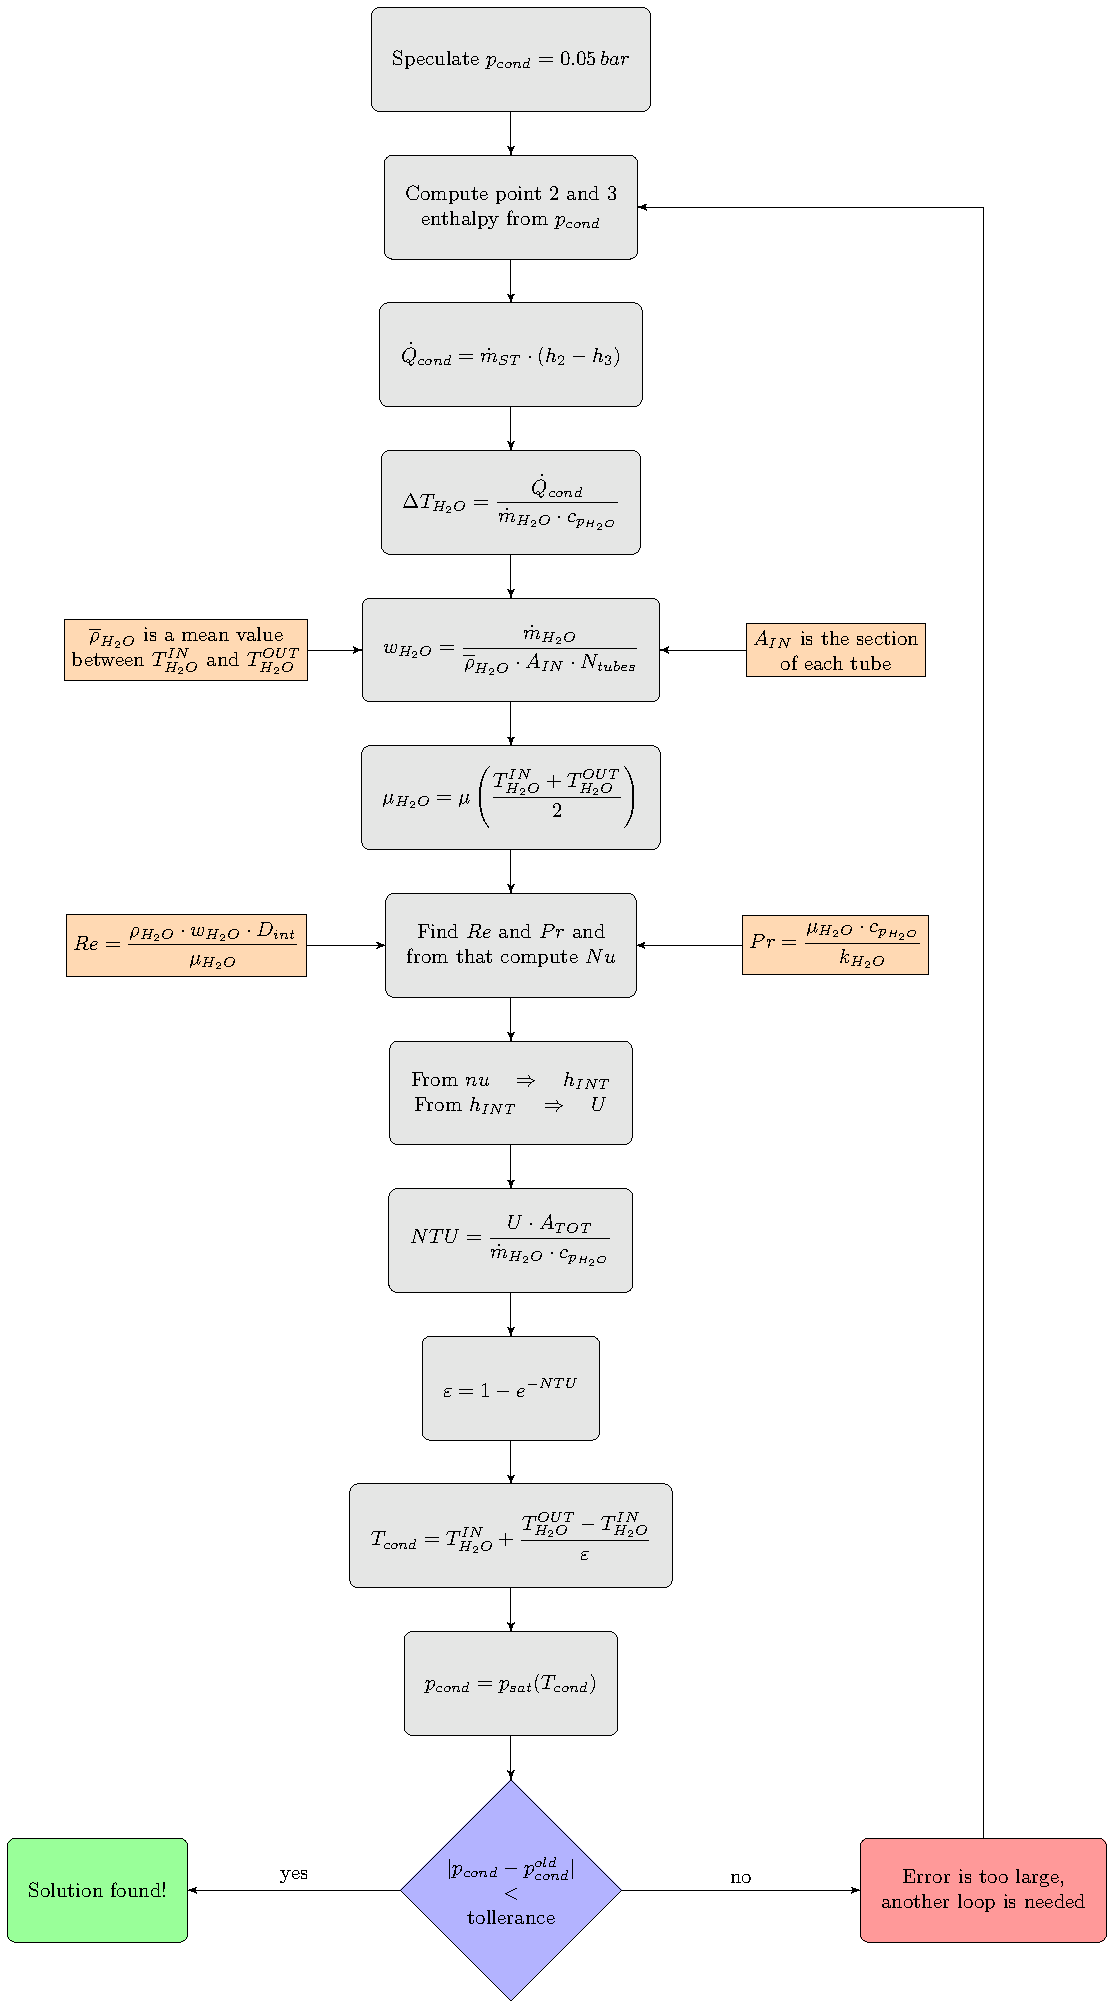
\includegraphics[width=0.85\textwidth]{img/diagram_fig.pdf}
\caption{Iterative Algorithm.}
\end{figure}

The algorithm's operation is simple: starting from the initial value of the crack, it evaluates, for both points A and C, the \emph{$\Delta K_A$} and \emph{$\Delta K_C$} and, thanks to the Paris' law, it updates the crack size \emph{$\text{a}_{i+1}$} at each cycle. Then, if the $\Delta K_{i-th}$ value is lower than \emph{$\text{K}_{IC}$}, the loop continues to increase the crack size; instead, if the $\Delta K_{i-th}$ is higher than \emph{$\text{K}_{IC}$}, there loop stops, due to the fact that the will be an unstable crack propagation (burst condition). Moreover, the loop can also stop when the crack depth  \emph{$\text{a}_{i-th}$} reaches the $95\perc$ of the shell thickness (leakage before break condition).\\

The result which we have obtained is that the number of cycles at which the crack depth reaches the $95\perc$ of the shell thickness  are $\round{15764}$.\\
In figure \ref{crack_propagation}, it is shown the crack propagation's shape; each line represents a time shift of 222 cycles. As we can notice in agreement with the theory, the tips of the shallow crack propagate with different speed and after a sufficient number of cycles the crack shape becomes quasi semi-circular.
\begin{figure}[H]
\centering
\includegraphics[width=0.75\textwidth]{img/crack_propagation.pdf}
\caption{Crack Propagation.}
\label{crack_propagation}
\end{figure}

\begin{figure}[H]
\centering
\includegraphics[width=0.75\textwidth]{img/crack_propagation_plot.pdf}
\caption{Crack Propagation Plot.}
\label{crack_propagation plot}
\end{figure}


\subsection{Static Assessment considering a\\ Completely Through-Thickness Crack}


Now, we have to make the static assessment considering a completely through-thickness defect; actually, a crack depth is is reasonable to consider  as a completely through-thickness defect, if it has reached the $95\perc$ of the shell thickness 
In addition to that,we will use as pressure value \textbf{two} times the nominal pressure, as a safety factor.

The standard provides the way by which the Stress Intensity Factor should be calculated.
\begin{equation}
\text{K}= \beta\, \text{f}_w \cdot \sigma \, \sqrt{\pi\,a}
\end{equation}
\begin{conditions}
\text{f}_w  & $\dfrac{1}{\sqrt{\cos \left(  \dfrac{\pi\,a}{w} \right) }}$   \\[2.5em]
\beta & $\sqrt{1 + 3.2\, \dfrac{a^2}{2\,\text{r}_m\cdot t}}$\\[1em]
\sigma & hoop stress with $p = 1.5 \cdot p_\text{nom} = 30 \,\text{bar}$;\\[0.5em]
a & is the semi-width of the crack when the depth reaches $95\perc$ of the shell thickness.\\[0.5em]
\text{r}_m & is the average shell radius equal to $\round{112.1000}\mm$.\\[0.5em]
\text{t} & is the shell thickness.\\[0.5em]
\end{conditions}

Applying the previous equation we obtain the stress intensity factor that values $\round{124.6847} \MPam$.
Since the limit of the material is $\text{K}_{IC} = 200 \MPam$ that is greater than $\text{K}_I$ the static assessment with a crack through the thickness is satisfied.

%$\dfrac{\text{da}}{\text{dN}}$ = $\text{C}\, \Delta K ^\text{m}$





\end{document}